% ======================================================================
% STAGE-1 REPORT  — parallel deliverable and thesis Chapter-3 seed.
% Compile: pdflatex stage1_report.tex  (Overleaf: just upload folder)
% Equations come from ../equations/equations_master.tex — edit THERE.
% Figures come from the repo experiment folder — regenerable, never pasted.
% ======================================================================
\documentclass[11pt,a4paper]{article}
\usepackage[margin=2.5cm]{geometry}
\usepackage{amsmath,amssymb,graphicx,booktabs,siunitx,hyperref}
\usepackage{times}                       % Times text; CM math = IEEE look
\graphicspath{{../../experiments/2026-07-07_stage1_final/figures/}{../../thesis/figures/}}
% ======================================================================
% EQUATIONS MASTER - single source of truth for every project equation.
% Used by: (1) render_equations.py  -> slide PNGs (Computer Modern)
%          (2) \input into report/thesis LaTeX -> native journal math
% Rule: an equation exists HERE or it does not exist. Edit here only.
% ======================================================================

% --- E1: the core residual idea ---------------------------------------
\newcommand{\eqCore}{%
\tau_{\mathrm{load}}(t) \;=\; \tau_{\mathrm{measured}}(t) \;-\; \tau_{\mathrm{model}}(t)}

% --- E2: Euler-Lagrange operator ---------------------------------------
\newcommand{\eqEL}{%
\frac{d}{dt}\left(\frac{\partial L}{\partial \dot{q}_i}\right) - \frac{\partial L}{\partial q_i} \;=\; \tau_i}

% --- E3: manipulator form ----------------------------------------------
\newcommand{\eqManip}{%
D(q)\,\ddot{q} \;+\; C(q,\dot{q})\,\dot{q} \;+\; f_v\,\dot{q} \;+\; f_c\,\mathrm{sgn}(\dot{q}) \;+\; G(q) \;=\; \tau}

% --- E4: saddle (revolute) equation ------------------------------------
\newcommand{\eqSaddle}{%
\tau_3 \;=\; (I_{zz} + M_d r^2)\ddot{q}_3 \;+\; 2 M_d r\,\dot{d}_4\,\dot{q}_3 \;+\; M_d\,g\,r\cos q_3 \;+\; f_{v3}\,\dot{q}_3}

% --- E5: crowd (prismatic) equation ------------------------------------
\newcommand{\eqCrowd}{%
F_4 \;=\; M_d\,\ddot{d}_4 \;-\; M_d r\,\dot{q}_3^{\,2} \;+\; M_d\,g\sin q_3 \;+\; f_{v4}\,\dot{d}_4}

% --- E6: time-varying lever arm ----------------------------------------
\newcommand{\eqLever}{%
r(t) \;=\; d_4(t) + c, \qquad c = x_{\mathrm{ref}} - L_{\mathrm{COG}} = -1.32\ \mathrm{m}}

% --- E7: linear-in-parameters regressor --------------------------------
\newcommand{\eqRegressor}{%
\tau \;=\; Y(q,\dot{q},\ddot{q})\,\theta, \qquad \theta = [\,m,\; mc,\; mc^2+I_{zz},\; f_v,\; f_c\,]^{\top}}

% --- E8: least squares + covariance ------------------------------------
\newcommand{\eqLS}{%
\hat{\theta} = (Y^{\top}Y)^{-1} Y^{\top}\tau, \qquad \mathrm{Cov}(\hat{\theta}) = \hat{\sigma}^2 (Y^{\top}Y)^{-1}}

% --- E9: goodness-of-fit metrics (Fu 2022 Eq. 18 convention) -----------
\newcommand{\eqMetrics}{%
R^2 = 1 - \frac{\sum_k (\tau_k - \hat{\tau}_k)^2}{\sum_k (\tau_k - \bar{\tau})^2}, \qquad \mathrm{RMSE} = \sqrt{\frac{1}{N}\sum_k (\tau_k - \hat{\tau}_k)^2}}

% --- E10: HPINN hybrid loss (Fu 2022, Eqs. 11-15) ----------------------
\newcommand{\eqHPINN}{%
J \;=\; \alpha\, J_{\mathrm{dynamics}} \;+\; \eta\, J_{\mathrm{energy}}}
    % SINGLE SOURCE of every equation

\title{Dynamic Modelling and Verified Identification of a 2-DOF Cable-Shovel
       Subsystem:\\ Stage-1 Report}
\author{Suhail Majeed Sheikh \\ \small JRF, Dept.\ of Mining Engineering, IIT Kharagpur
        \\ \small Project IIT/SRIC/R/AEH/2026/104 (CMPDI) \quad Supervisor: Dr.\ Sunita Das Mishra}
\date{July 2026}

\begin{document}\maketitle

\begin{abstract}
This report documents Stage 1 of the load-torque--estimation programme:
derivation of the two-degree-of-freedom dynamics of the shovel saddle--crowd
subsystem, verification against an independent multibody simulation to machine
precision, and exact blind recovery of all physical parameters. The validated
model constitutes the subtraction reference required for instantaneous
load-torque estimation, the enabling quantity for drive health management.
\end{abstract}

% ----------------------------------------------------------------------
\section{Problem statement and approach}          % <- WU1
Health monitoring of shovel drives from motor signatures requires separating
three contributions to motor torque: rigid-body motion, external load, and
machine condition. The programme's central quantity is therefore
\begin{equation}\eqCore\label{eq:core}\end{equation}
which demands a motion model exact enough that its residual contains only
load and condition effects. Payload estimation follows as a byproduct of the
same channel.
% TODO(WU1): expand health-first motivation, cite downtime economics.

% ----------------------------------------------------------------------
\section{Dynamic model}                            % <- WU3, WU4
\subsection{Kinematic abstraction}
% TODO(WU3): 2-DOF abstraction figure + frames; refer anatomy figure.
The lever arm from pivot to the body's centre of mass is time-varying:
\begin{equation}\eqLever\label{eq:lever}\end{equation}

\subsection{Equations of motion}
Applying the Euler--Lagrange operator
\begin{equation}\eqEL\label{eq:el}\end{equation}
to the kinetic and potential energies of the dipper--handle body, and
appending non-conservative friction, yields the manipulator form
\begin{equation}\eqManip\label{eq:manip}\end{equation}
whose two scalar components are the saddle equation
\begin{equation}\eqSaddle\label{eq:saddle}\end{equation}
and the crowd equation
\begin{equation}\eqCrowd\label{eq:crowd}\end{equation}
% TODO(WU4): full derivation steps (thesis version); term-by-term physical
% reading (inertia / Coriolis / gravity leverage / friction).

% ----------------------------------------------------------------------
\section{Verification methodology}                 % <- WU5, WU6
% TODO(WU5): Simscape oracle description; non-circularity argument.
% TODO(WU6): isolation protocol - g=0 test, frequency-doubling signature,
%            perfect-fit-wrong-parameters deduction. (research_log 2026-07-06)

% ----------------------------------------------------------------------
\section{Parameter identification}                 % <- WU7, WU8
All parameters are the published values of Rasuli \emph{et al.}\ Table II.
Identification uses the linear-in-parameters regrouping
\begin{equation}\eqRegressor\label{eq:regressor}\end{equation}
solved by ordinary least squares with covariance-based confidence intervals:
\begin{equation}\eqLS\label{eq:ls}\end{equation}
Goodness of fit is reported by the field-standard metrics
\begin{equation}\eqMetrics\label{eq:metrics}\end{equation}
% TODO(WU8): identifiability analysis (gravity 2.5 MNm vs inertia 10 kNm),
%            conditioning story (d4 amplitude), CI reading rules.

% ----------------------------------------------------------------------
\section{Results}                                  % <- WU9
\begin{figure}[t]\centering
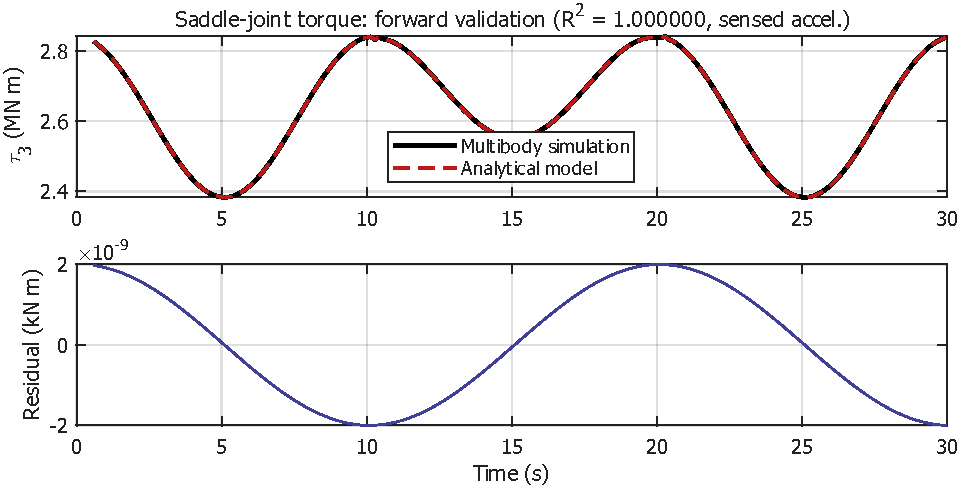
\includegraphics[width=\textwidth]{fig_B1_revolute_validation.pdf}
\caption{Forward validation of the saddle equation against the independent
multibody solution: $R^2 = 1.000000$, residual at the $10^{-13}$
floating-point floor.}\label{fig:b1}
\end{figure}
% TODO(WU9): results table (all five parameters exact, CIs ~0);
%            crowd-equation first validation; gradient-vs-sensed study (fig_C1)
%            and the 56% Izz bias finding -> instrumentation requirement.

\section{Scope and outlook}                        % <- WU10 + roadmap
% TODO: honest-scope statements (machine precision = mathematical correctness;
%       zero-width CIs are simulation-only), M2 design + acceptance criterion.

\begin{thebibliography}{9}\small
\bibitem{rasuli2014} A.~Rasuli, S.~Tafazoli, W.~G.~Dunford,
``Dynamic modeling, parameter identification, and payload estimation of
mining cable shovels,'' \emph{IEEE Trans.\ Ind.\ Appl.}, 50(3), 2014.
\bibitem{fu2022} T.~Fu \emph{et al.}, ``Dig-load prediction of electric cable
shovel based on hybrid physics-informed neural network,''
\emph{Chin.\ J.\ Mech.\ Eng.}, 35, 2022.
\bibitem{tafazoli1999} S.~Tafazoli, P.~D.~Lawrence, S.~E.~Salcudean,
``Identification of inertial and friction parameters for excavator arms,''
\emph{IEEE Trans.\ Robot.\ Autom.}, 15(5), 1999.
\bibitem{frimpong2008} S.~Frimpong, Y.~Hu, ``Cable shovel digging dynamics
and simulation in oil sands excavation,'' 2008.
\end{thebibliography}
\end{document}
